\chapter{高频电外科发生器系统设计}
%
\section{引言}
高频电外科发生器作为典型的高频能量应用医疗设备，其系统设计涉及高频电能产生与调制、生物组织电学特性、功率控制策略等多个关键技术环节。为实现在复杂、动态生物负载条件下对输出能量的安全、稳定和精确控制，有必要从工作机理、负载特性以及系统功能需求等多个层面对高频电外科系统进行分析与设计。

本章首先对高频电外科发生器的基本工作原理进行阐述，分析高频电能在生物组织中的作用机理与常见工作模式的差别和应用场景，为后续系统设计奠定理论基础。随后，对生物组织在高频能量作用下呈现出的频率相关性及非线性阻抗变化特性进行分析，为功率控制与优化策略的选择提供依据。在此基础上，结合相关标准以及临床手术需求明确系统的设计指标与功能配置。进一步地，从工程实现与控制性能的角度，对多种高频逆变拓扑和常见调功方式进行对比分析，确定适用于本系统的逆变与输出功率调节方案。最后，在上述分析的基础上，给出高频电外科发生器的总体系统方案设计，为后续硬件电路设计与控制算法实现提供整体架构与技术路线。

\section{高频电外科发生器工作原理}
高频电外科发生器又称高频电刀，是一种广泛应用于各类电外科手术中的大功率高频能量发生器，其核心工作原理是将工频市电的低频电能经过变频变压、功率放大转换为作用于人体的高频高压电能（频率通常在200KHz至5MHz之间），利用高频电流流经人体组织时产生的热效应实现对手术部位的切割和凝血。从微观层面看，电极与组织的有效接触面积小，在接触点形成极大的电流密度，细胞内的大量带电粒子（如钠、钾粒子）在高频交变电场的作用下发生高速振荡，离子间的摩擦和碰撞产生大量热量，根据传递热量与达到的温度不同，产生组织脱水、汽化和蛋白质变性的医疗效果：当温度低于45℃时，细胞热损伤可逆；组织温度达到60℃-90℃时，细胞内水分缓慢蒸发，蛋白质分子间的化学键断裂，导致组织凝固收缩从而实现止血和血管闭合的效果；当组织温度上升到100℃以上时，细胞内液瞬间沸腾汽化，体积剧烈膨胀导致细胞膜破裂，在宏观上形成组织分离的效果，同时伴随有细胞内物质变为烟雾释放到环境中；若温度继续升高到200℃以上，组织发生碳化并形成烧焦的黑色痂皮，影响伤口愈合并增加感染风险。

电外科发生器输出信号的频率设定至关重要，这主要源于生物组织对不同频率的电流的响应存在显著差异。低频电流流经人体会引发法拉第效应，在产生热效应的同时导致神经和肌肉产生去极化，引起强烈的肌肉痉挛或心室纤颤，严重时会危及患者生命安全。然而，当电流频率超过200kHz或300kHz时，由于电流极性变化的周期极短，带电离子无法在细胞膜两侧产生足够的离子迁移和去极化，神经肌肉刺激效应基本消失，取而代之的是热效应占据主导地位。因此高频电外科发生器的输出频率一般设计在300kHz以上，以确保手术过程中的安全性和有效性。此外，高频电流在组织中流动时产生交变的磁场，磁场感应的电流会进一步影响组织内电流的分布，使电流倾向于在组织表层流动，减少对人体深层内脏器官的损伤。以上生物组织的集肤效应和热效应、法拉第效应共同构成了高频电外科发生器
切割和凝血两大基本功能的理论基础。

\begin{figure}[htbp]
\centering
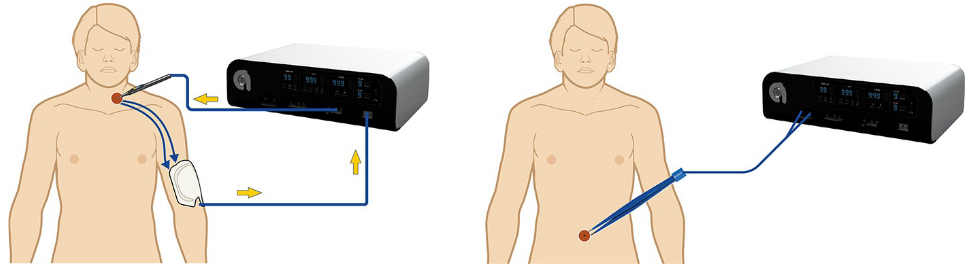
\includegraphics[scale=0.63]{Fig/monobi.png}
\caption{\label{monobi}单双极模式下的电外科手术系统}
\end{figure}

电外科发生器产生的高频能量需要通过手术电极装置作用在患者组织处才能产生理想的医疗效果，根据手术电极的输出方式、数量以及电流回路的构成方式的不同，高频电外科发生器的工作模式可分为单极模式和双极模式，如图\ref{monobi}所示。在单极模式下，电外科发生器产生的高频电流经发生器、手术电缆、单极刀头、患者组织、负极板后返回发生器，构成完整的电流回路。不同于手术电极，负极板与患者表面皮肤的接触面积较大，为高频电流提供低阻抗和低电流密度的返回通道，从而避免对患者造成局部损伤。相比之下，双极模式的高频电流仅在双极镊的两个夹持端之间流动，无需负极板收集电流，同时高频电流在患者体内的流通路径短，配合手动施加压力可实现更好的组织凝固效果，具有更高的安全性和更小的热损伤。单极模式通常输出功率较高，常用于大面积组织切割、干燥以及止血，而双极模式则因其安全性和精确性优势，通常用于精细化治疗中的组织凝血和血管闭合。

\begin{figure}[htbp]
\centering
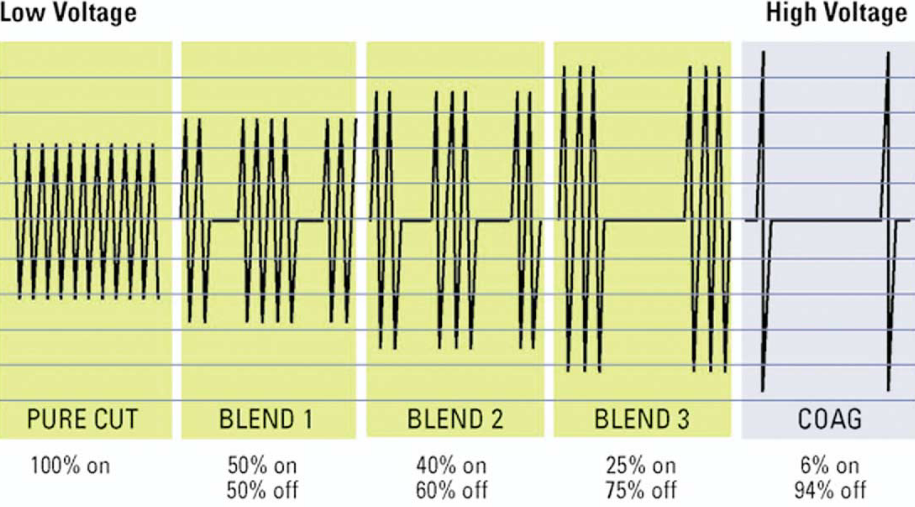
\includegraphics[scale=0.63]{Fig/crestfactor.png}
\caption{\label{crestfactor}不同波峰因子的输出波形\cite{massarwehElectrosurgeryHistoryPrinciples2006}}
\end{figure}

为了实现不同的临床手术效果，高频电外科发生器通过调制输出电压的波形来控制能量输出的形式，如图\ref{crestfactor}所示。波峰因子是衡量输出波形特性的关键指标，为输出信号峰值与其均方根值的比值。在纯切模式下，发生器输出连续的等幅正弦波，波峰因子较低（1.4-2.0），能够连续提供较高的平均功率，适用于组织的快速切割和蒸发；而在电凝模式下，发生器输出高波峰因子（通常>5.0）的间断性脉冲波形，在脉冲间隙允许组织冷却，其输出峰值电压非常高但平均功率较低，主要引发组织脱水和凝固，甚至产生电火花进行非接触式的喷射凝血。现代高频电外科发生器通常具有多种不同波峰因子的输出模式，如纯切、混切、电灼、电凝和喷凝等模式，通过调整有效输出与间断时间的比例，在复杂手术环境下为医生提供多样化的手术作用效果选择。

\begin{figure}[htbp]
\centering
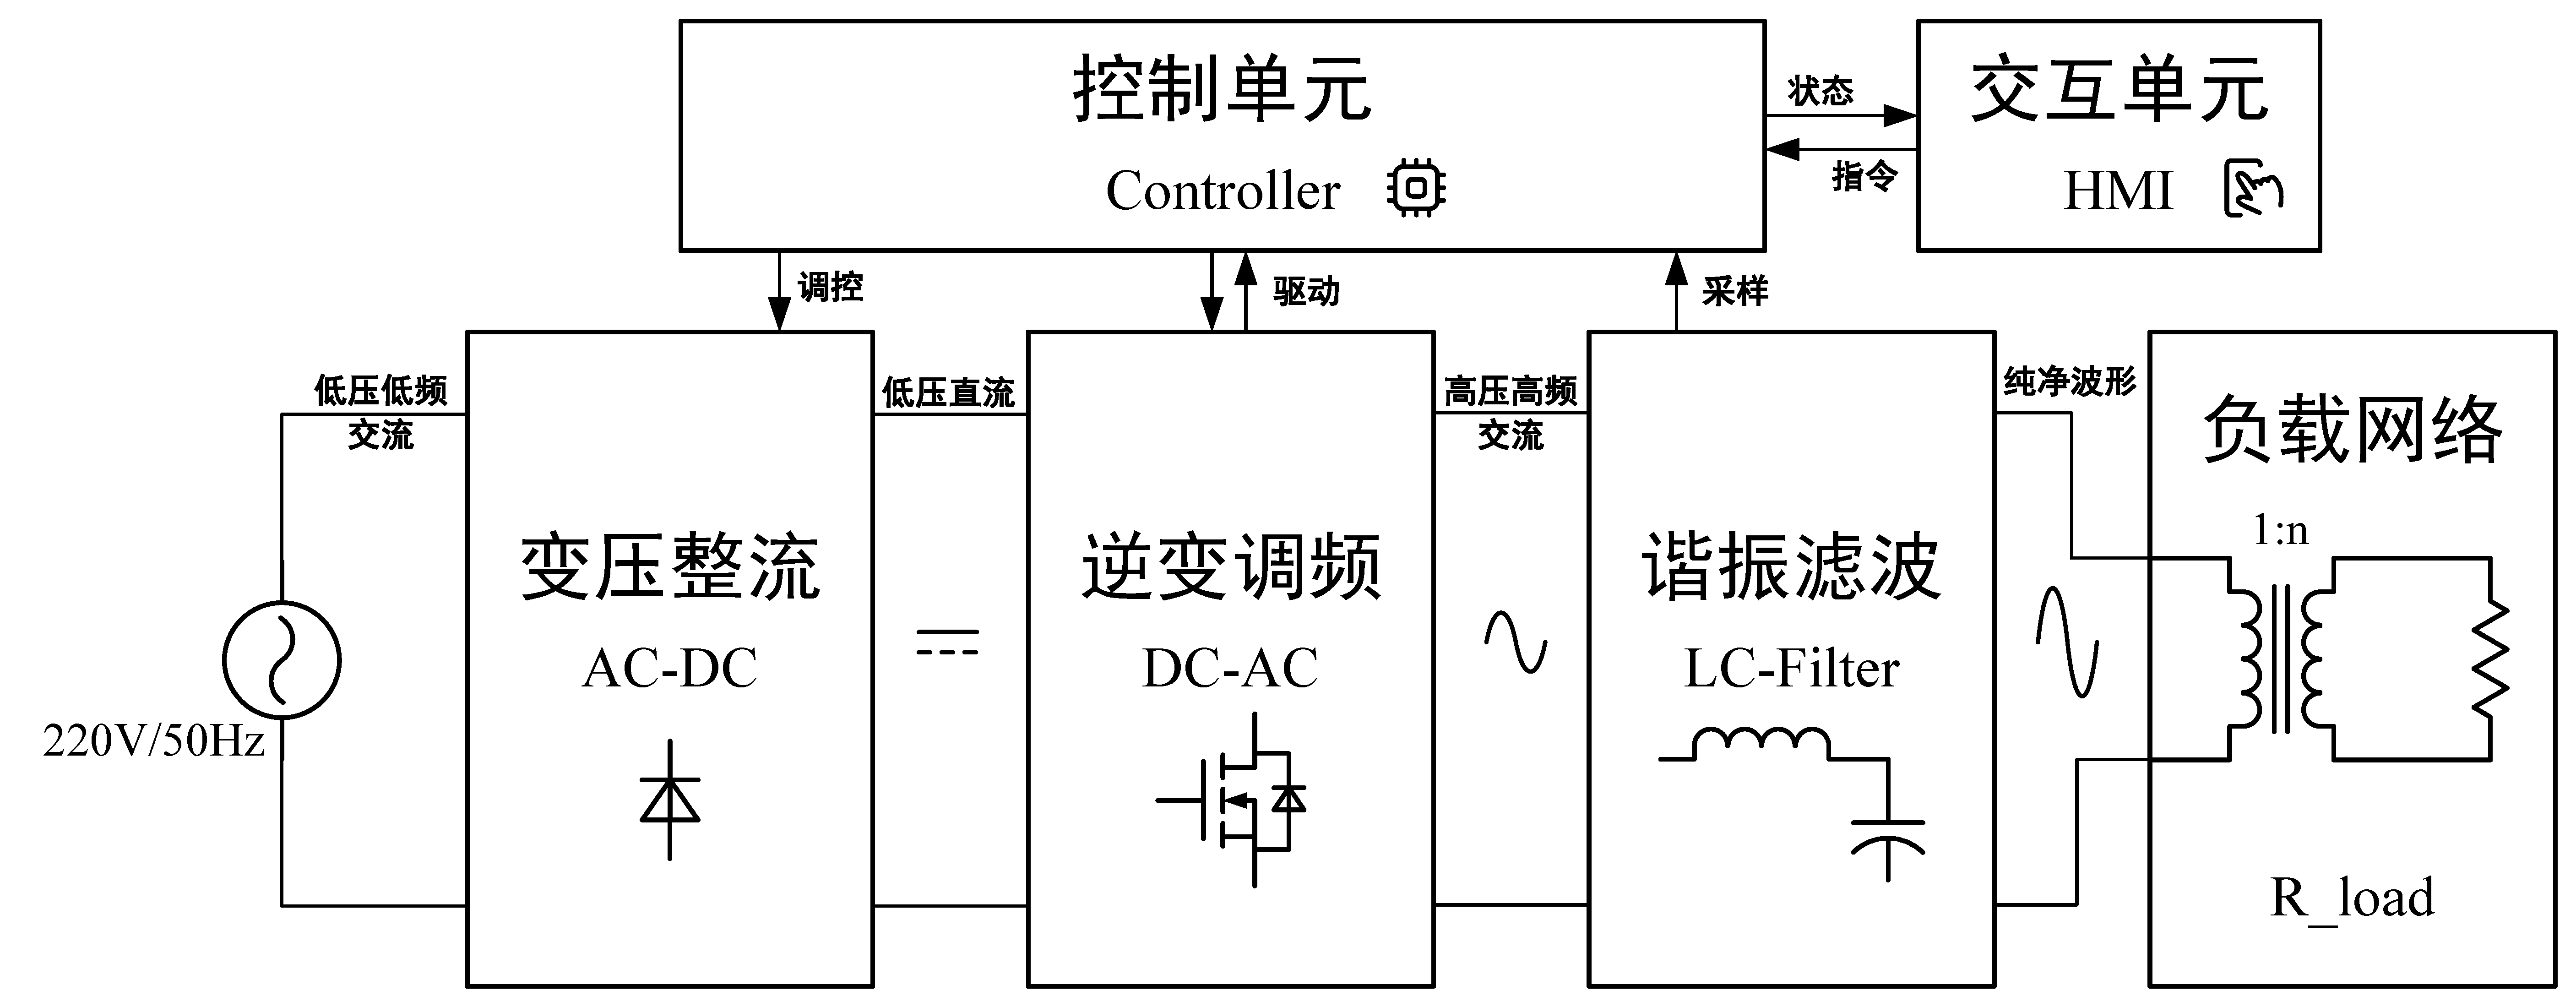
\includegraphics[scale=0.15]{Fig/briefsystem.pdf}
\caption{\label{briefsystem}高频电外科发生器系统结构框图}
\end{figure}

常见的高频电外科发生器系统拓扑结构框图如图\ref{briefsystem}所示。其中，市电经变压整流模块完成AC/DC转换，得到可调低压直流电源为后级电路提供稳定的直流馈电，同时也作为系统的主要功率来源；逆变调频模块在此基础上对直流电能进行高频逆变与调制，实现200KHz-5MHz范围内的高频交流信号输出，并通过谐振滤波模块对输出信号进行选频和波形整形，以获得满足手术需求的高频正弦电压波形；经滤波后的纯净交流正弦信号经过高频变压器实现电气隔离和电压升压后输出至手术电极，从而完成向生物组织的高频能量传递；系统控制单元对能量发生主拓扑电路进行调控和驱动，同时对关键电压、电流等参数进行采样与监测，并与交互单元进行数据交互，实现系统工作状态显示及操作者指令的接收与执行。

\section{生物组织阻抗特性}
在电外科手术中，人体生物组织作为高频电外科发生器输出回路的最终负载，其阻抗特性直接影响系统工作状态和手术效果，研究和分析组织阻抗模型不仅有助于系统参数和架构设计，还为系统的控制算法优化提供理论基础。

生物组织的基本单位是细胞，人体细胞浸泡在体液中，细胞内外液含有大量的带电离子，（如$\mathrm{Na}^+$、$\mathrm{K}^+$、$\mathrm{Cl}^-$等），同时也存在一些细胞外间质和胶状物质，在电学上表现为电阻特性。而包裹细胞的细胞膜则由磷脂双分子层构成，表现为电容特性，随着频率的升高细胞膜的电容效应逐渐减弱。因此生物组织的阻抗在外加交变电场作用下表现为由电阻（实部）和容抗（虚部）组成的复阻抗，其数值随激励电流频率呈现显著的非线性和频散特性。此外，不同类型的组织（如肌肉、脂肪、骨骼等）由于其结构和成分的差异，阻抗特性也具有较大差异。

\begin{figure}[htbp]
\centering
\begin{minipage}[c]{0.5\textwidth}
\centering
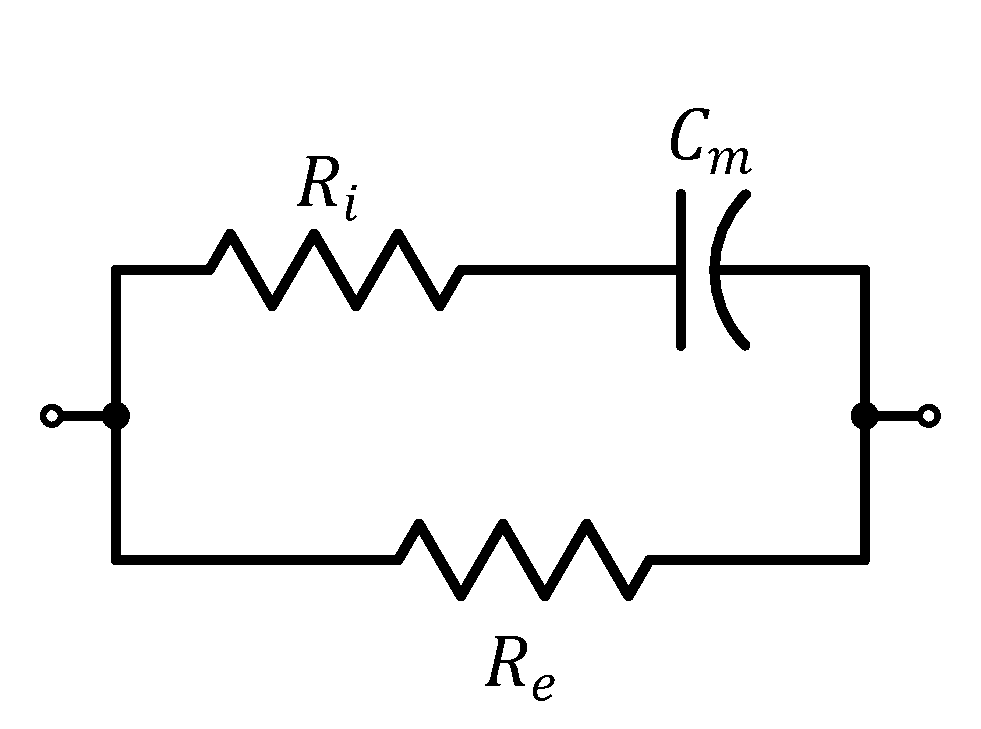
\includegraphics[scale=0.25]{Fig/2r1c.pdf} %1:1导入
\end{minipage}%
\begin{minipage}[c]{0.5\textwidth}
\centering
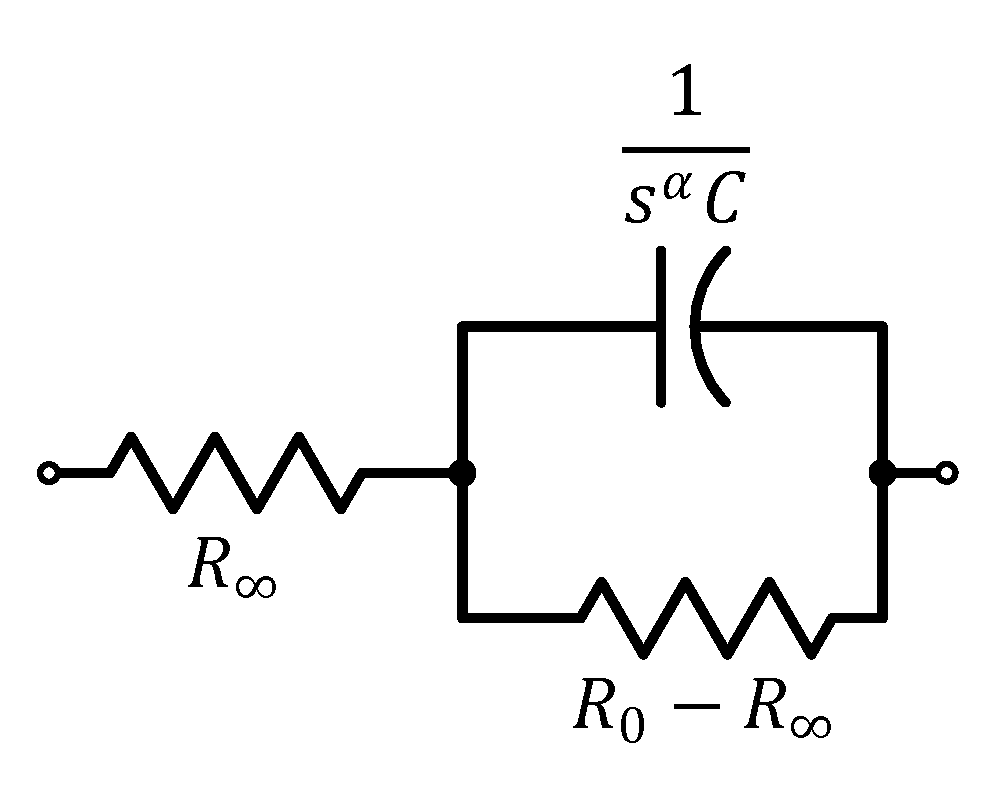
\includegraphics[scale=0.25]{Fig/cole.pdf}
\end{minipage}\\[1pt]
\begin{minipage}[t]{0.5\textwidth} % 以下为新添加页面划分，[t]表示行顶部对齐
\caption{\label{2r1c}2R1C生物组织阻抗模型}
\end{minipage}%
\begin{minipage}[t]{0.5\textwidth}
\caption{\label{cole}Cole生物组织阻抗模型}
\end{minipage}\\[10pt]
\begin{minipage}[c]{1.0\textwidth}
\centering
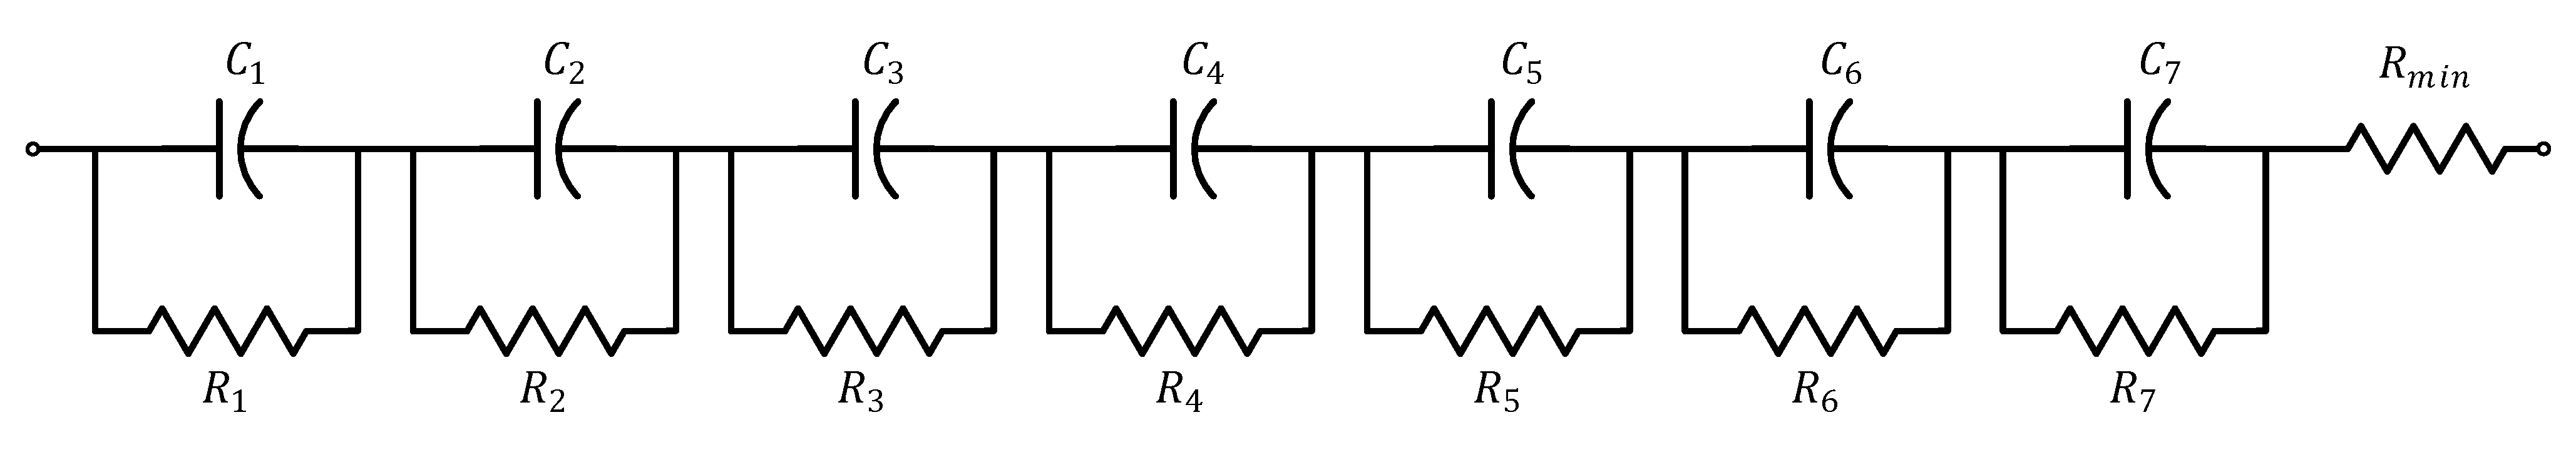
\includegraphics[scale=0.25]{Fig/belik.pdf}
\end{minipage}\\[1pt]
\begin{minipage}[t]{1.0\textwidth} % 以下为新添加页面划分，[t]表示行顶部对齐
\caption{\label{belik}七元件级联生物组织阻抗模型}
\end{minipage}%
\end{figure}

在此基础上，国内外学者提出了多种等效电路模型用于描述生物组织的阻抗特性。Fricke提出的2R1C模型能够较好地描述低频范围内的阻抗特性，如图\ref{2r1c}所示。其中$R_e$为细胞外液的电阻，$R_i$为细胞内液的电阻，$C_m$为细胞膜的并联电容。2R1C模型的复阻抗可表示为：
\begin{equation}
    Z=R_\mathrm{e}\parallel(R_i+X_c)=\frac{R_\mathrm{e}(1+R_ij\omega C_m)}{1+j\omega C_m(R_\mathrm{e}+R_i)}, \omega=2\pi f
\end{equation}

七元件级联模型由Dornhof和Belik提出，是三元件RC模型的扩展，旨在通过SPICE仿真更精确地模拟生物组织在1kHz至1MHz宽频带内的阻抗特性\cite{dornhofElectricalCircuitBiological2019}，其等效电路模型\ref{belik}所示。在该电路中，电容值根据双曲余割函数计算和分布，并按照从左至右递减的顺序排列，从而更紧密地拟合猪肉肌肉和肝脏组织的实测阻抗谱曲线。


Cole模型最早由Kenneth S.Cole提出，旨在全面描述生物组织或细胞悬液复阻抗的频率依赖性行为，其等效电路描述如图\ref{cole}所示。其中在低频极限下，细胞膜电容呈现高阻抗，电流主要流经细胞外液，使用$R_0$表示细胞外液的电阻；在高频条件下，细胞膜电容效应逐渐减弱，电流可同时流经细胞内外液，使用$R_\infty$表示细胞内液与细胞外液的并联电阻；$C$并非理想电容，而是表现出分数阶特性的恒相元件（CPE），其电压电流关系使用分数阶微分方程表述：$i(t)=C({d^\alpha v(t)}/{dt^\alpha})$，电气特性介于纯电阻和理想电容之间；$\alpha$为分数阶次或分布系数，反映了细胞膜形态分布的非均匀性和膜电容的分散性，$\alpha=1$时退化为经典的Fricke/2R1C模型。Cole模型的复阻抗可表示为：
\begin{equation}
    Z=R_{\infty}+\frac{R_1}{1+(j\omega)^{\alpha}R_{1}C}
\end{equation}

在特定参数下绘制Cole模型的奈瑞斯特图如图\ref{coleplot}所示。可以看出，与传统的理想线性电路模型（$\alpha = 1$）不同，Cole模型（$0<\alpha<1$）的阻抗轨迹在复平面上近似表现为圆心在实轴之下的半圆弧形，其圆心下沉角为$\theta = {\alpha\pi}/2 $，随着频率的升高，复阻抗从$R_0$逐渐过渡到$R_\infty$。由此可见，Cole模型通过引入分布参数$\alpha$，有效描述了生物组织的非理想、非均匀的电学结构。根据实验测定，生物组织中$\alpha$的取值范围通常在0.6至0.9之间，具体数值依赖于组织类型和测量条件\cite{freebornColeImpedanceModelRepresentations2021}。

\begin{figure}[htbp]
\centering
\begin{minipage}[c]{0.5\textwidth}
\centering
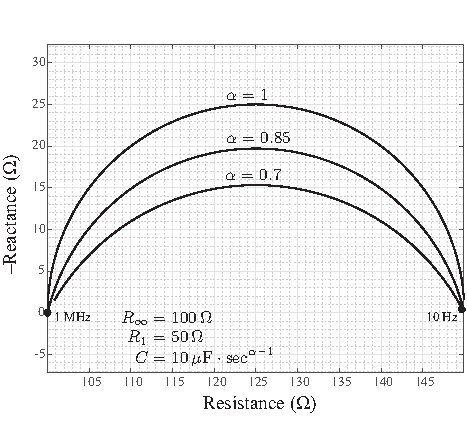
\includegraphics[scale=1.0]{Fig/cole-plot.pdf} %1:1导入
\end{minipage}%
\begin{minipage}[c]{0.5\textwidth}
\centering
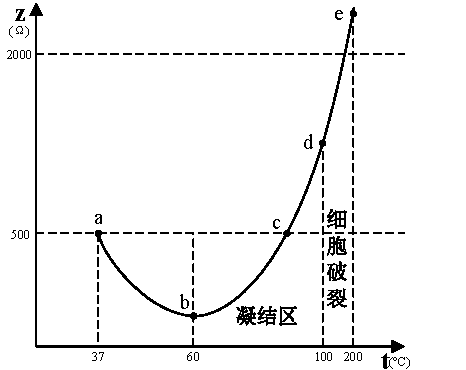
\includegraphics[scale=1.0]{Fig/impedchange.pdf}
\end{minipage}\\[1pt]
\begin{minipage}[t]{0.5\textwidth} % 以下为新添加页面划分，[t]表示行顶部对齐
\caption{\label{coleplot}Cole模型在特定参数下的奈奎斯特图}
\end{minipage}%
\begin{minipage}[t]{0.5\textwidth}
\caption{\label{impedchange}生物组织阻抗-温度变化曲线}
\end{minipage}%
\end{figure}

高频电能作用于生物组织时，由于组织阻抗转换为热能，导致组织内水分蒸发和细胞结构破坏，进而引起阻抗的显著变化。已有实验研究表明，在组织闭合过程中随着高频能量作用时间的延长，生物组织阻抗的奈奎斯特曲线半径持续增大，且曲线中心逐渐向右侧移动，表明组织在各频率范围内的阻值均呈现上升趋势\cite{YanBoWenDianWaiKeShePinNengLiangFaShengQiKongZhiXiTongDeYanZhi2014}。此外，生物组织在手术过程中的阻抗-温度关系通常呈现明显的非线性特征，如图\ref{impedchange}所示：在加热初期（约37°C至60°C之间），随着温度升高细胞膜通透性增加，离子迁移加快，组织阻抗略有下降；当温度进入凝结区间（60°C至90°C之间），组织逐渐脱水且蛋白质发生变性，阻抗开始缓慢回升；当温度超过100°C时，组织内水分大量蒸发，细胞膜破裂导致组织迅速脱水干燥，阻抗值急剧上升；若温度进一步升高并超过200°C则组织发生碳化并形成烧焦痂皮，阻抗将达到极高水平。

\begin{table}[htbp]
    \caption{\label{imped}常见人体组织的近似阻抗值}
    \centering
    \small
    \setlength{\tabcolsep}{20pt}
	\begin{tabular}{ c c c c }
        \hline
        组织 & 阻抗值 & 组织 & 阻抗值\\
        \hline
        血液            &  160Ω  & 肺脏 &  150-2000Ω\\
        肌肉、肾脏、心脏  &  200Ω  & 脂肪 &  3300Ω\\
        肝脏、脾脏     &  300Ω    & 粘膜 & 500Ω\\
        \hline
    \end{tabular}
\end{table}

表\ref{imped}总结了常见人体组织在典型工况下的阻抗取值范围。综合前述生物组织阻抗模型及其随频率与温度的变化过程，在高频电外科发生器的设计过程中需要充分考虑生物组织阻抗的动态变化特性，从而保证系统运行的稳定性及输出功率调节的准确性。

\section{设计指标及功能配置}
高频电外科发生器设计指标与功能配置是系统方案设计的基础，其设计参数选取的首要依据是国家医疗器械的相关标准，并结合临床手术的实际需求以及现有业界成熟产品参数综合确定。中华人民共和国国家标准GB9706.202-2021——《医用电气设备 第2-2部分:高频手术设备及高频附件的基本安全和基本性能专用要求》中，对高频手术设备的工作频率范围、输出功率精度以及故障保护机制等关键技术指标作出了明确规定\cite{GB97062022021YiYongDianQiSheBeiDi222021}。在此基础上，参考市场上主流高频电外科发生器产品的技术规格，如美国Valleylab公司的Force FX系列、德国Erbe公司的VIO系列以及国内上海沪通公司的GD系列，可进一步细化并明确设计指标，以满足不同场景下的多样化手术需求。

在功能模式方面，系统需具备单极和双极两种基本工作方式，并细分为多种手术模式以适应不同组织类型及手术目标对切割与凝血的性能要求。其中纯切模式输出连续正弦波，波峰因子较低，适用于清晰精确的平滑切割；电凝模式采用间断脉冲波形输出，波峰因子较高，主要用于组织凝固和止血；混切模式综合了纯切和电凝的输出特性，适用于需要同时切割和止血的手术场景；软凝模式则在输出控制上结合了功率控制与电压限幅控制的特点，在保证有效止血的同时最大程度降低组织碳化和电极粘连风险。

手术过程中输出功率的设定通常根依据手术类型（如神经外科、普通外科、泌尿外科）、组织特性（如肌肉、脂肪、血管）以及工作模式的进行综合调整。一般而言，单极模式下的大面积组织切割和快速止血对能量输入强度要求较高，而双极模式主要用于精细手术和小血管闭合，其功率设定限制在较小范围。根据临床实践经验，常见的高频电外科发生器输出功率调节范围设定在1至100W之间，以覆盖大部分常规手术需求。

综合上述分析以及前文对系统工作原理和生物组织阻抗特性的论述，本文所设计的高频电外科手术系统设计指标与功能配置如表\ref{index}所示。
\begin{table}[htbp]
    \caption{\label{index}高频电外科发生器设计指标}
    \centering
    \small
    \setlength{\tabcolsep}{20pt}
	\begin{tabular}{ c c c c }
        \hline
        性能指标 & 要求\\
        \hline
        输出频率     &  350KHz\\
        输出功率范围  &  1-100W\\
        额定负载     &  500Ω\\
        功率控制误差  &  $\leq$ 20\% \\
        输出模式     &  单双极；纯切、混切、电凝、软凝\\
        安全功能     &  极板连续性检测；过压、过流保护；短路保护\\
        \hline
    \end{tabular}
\end{table}

\section{调功方式选择}
在手术过程中对于不同类型的作用组织，需要设定不同的输出功率以平衡切割止血效果与组织损伤的关系，而输出功率的调节本质上是对单位时间内输出能量总量的调节。根据被调制变量的不同以及作用机制的差异，工程上逐步形成了以下几种成熟的调功方式：脉宽调制调功、脉宽移相调功、脉冲密度调功、脉冲均匀调制调功、调频调功以及直流调压调功：

\begin{enumerate}[topsep = 0 pt, itemsep= 0 pt, parsep=0pt, partopsep=0pt, leftmargin=44pt, itemindent=0pt, labelsep=6pt, label=(\arabic*)]
	\item 脉宽调制调功（PWM）：开关频率保持恒定，通过改变开关器件的导通占空比，从而调节输出的平均电压和电流，最终实现输出功率调节。PWM调功方式调制逻辑清晰，易于数字实现，但其在低占空比工况下开关损耗和死区效应对系统线性度的影响会进一步放大。
    \item 脉宽移相调功（PS-PWM）：开关频率和导通宽度保持恒定，通过调节不同桥臂开关管的相位偏移量，改变系统输出有效电压时间，进而实现功率控制。PS-PWM调功方式一般适用于全桥拓扑中，软件和电路实现较为复杂，但其在低占空比工况下的线性度优于PWM调功方式。
	\item 脉冲密度调功（PDM）/脉冲均匀调制调功（PUM）：脉冲宽度和幅值保持恒定，PDM调功通过改变单位时间内高电平脉冲的分布密度来调节输出功率，而PUM调功则通过改变单位时间内脉冲的个数来调节输出功率。两种调功方式均为有级调功，其输出功率响应不够平滑，且在负载较轻时容易出现电流断续。
	\item 调频调功（PFM）：占空比保持恒定，通过改变开关频率来调节输出功率。本质是通过改变系统工作点相对于谐振频率的位置，从而改变等效阻抗和能量传递效率。PFM调功轻载效率高、动态响应快，但其控制环路设计和参数整定复杂。
	\item 直流调压调功（DC）：从电源侧直接改变输入直流电压幅值的调功方式，输出功率通过电压—功率关系间接调整。DC调功实现较为简单直观，控制线性度高，但其依赖于前级可调直流电源质量，整体效率通常偏低。
\end{enumerate}

由于本文所设计的高频电外科发生器需具备较宽的输出功率调节范围，且需保证系统在轻载工况下仍具备良好的功率输出线性度，同时对系统响应的平滑性与控制器的易实现性有较高要求，因此本文选择使用直流调压调功方式。所设计系统使用可调直流电源作为逆变电路前级电源，通过控制开关电源中开关器件的导通时间调节输出电压。

\section{高频逆变电路拓扑选择}
根据前文对高频电外科发生器工作原理的分析可知，系统输入为220V、50Hz的交流市电，输出为频率350KHz的高压正弦波形。从电力电子技术的角度来看，高频电外科发生器系统本质上属于一种变频电源，常见的变频电源根据能量变换路径的不同可分为直接交-交变频和间接交-直-交变频两种。对于交-交变频结构，其工作在原理上依赖于器件的换流和输入电源频率，在低频大功率场合可具有较高的输出效率，但在高频应用中难以获得频率较高且谐波含量较低的正弦波输出。因此在高频电外科发生器系统应用中，广泛采用的是间接交-直-交变频拓扑结构。该拓扑通过前级AC/DC变换获得稳定直流母线电压，设计的核心集中于后级DC/AC逆变电路拓扑的设计。
\begin{figure}[htbp]
\centering
\begin{minipage}[c]{0.5\textwidth}
\centering
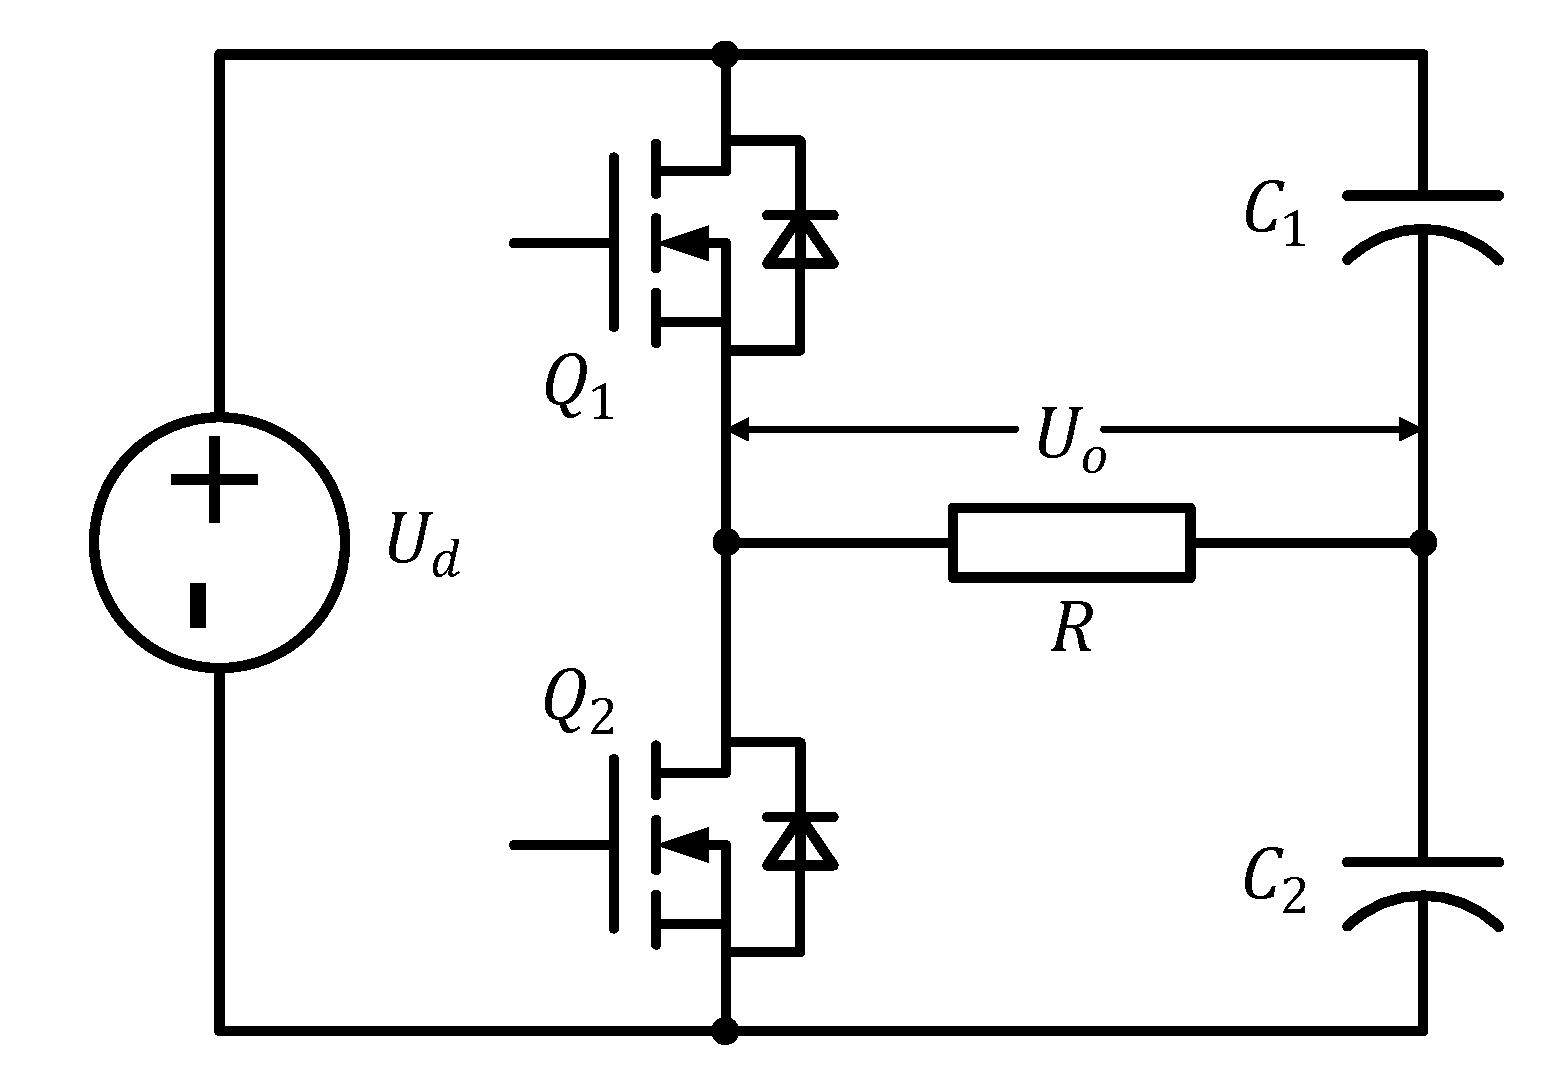
\includegraphics[scale=0.23]{Fig/halfbridge.pdf} %1:1导入
\end{minipage}%
\begin{minipage}[c]{0.5\textwidth}
\centering
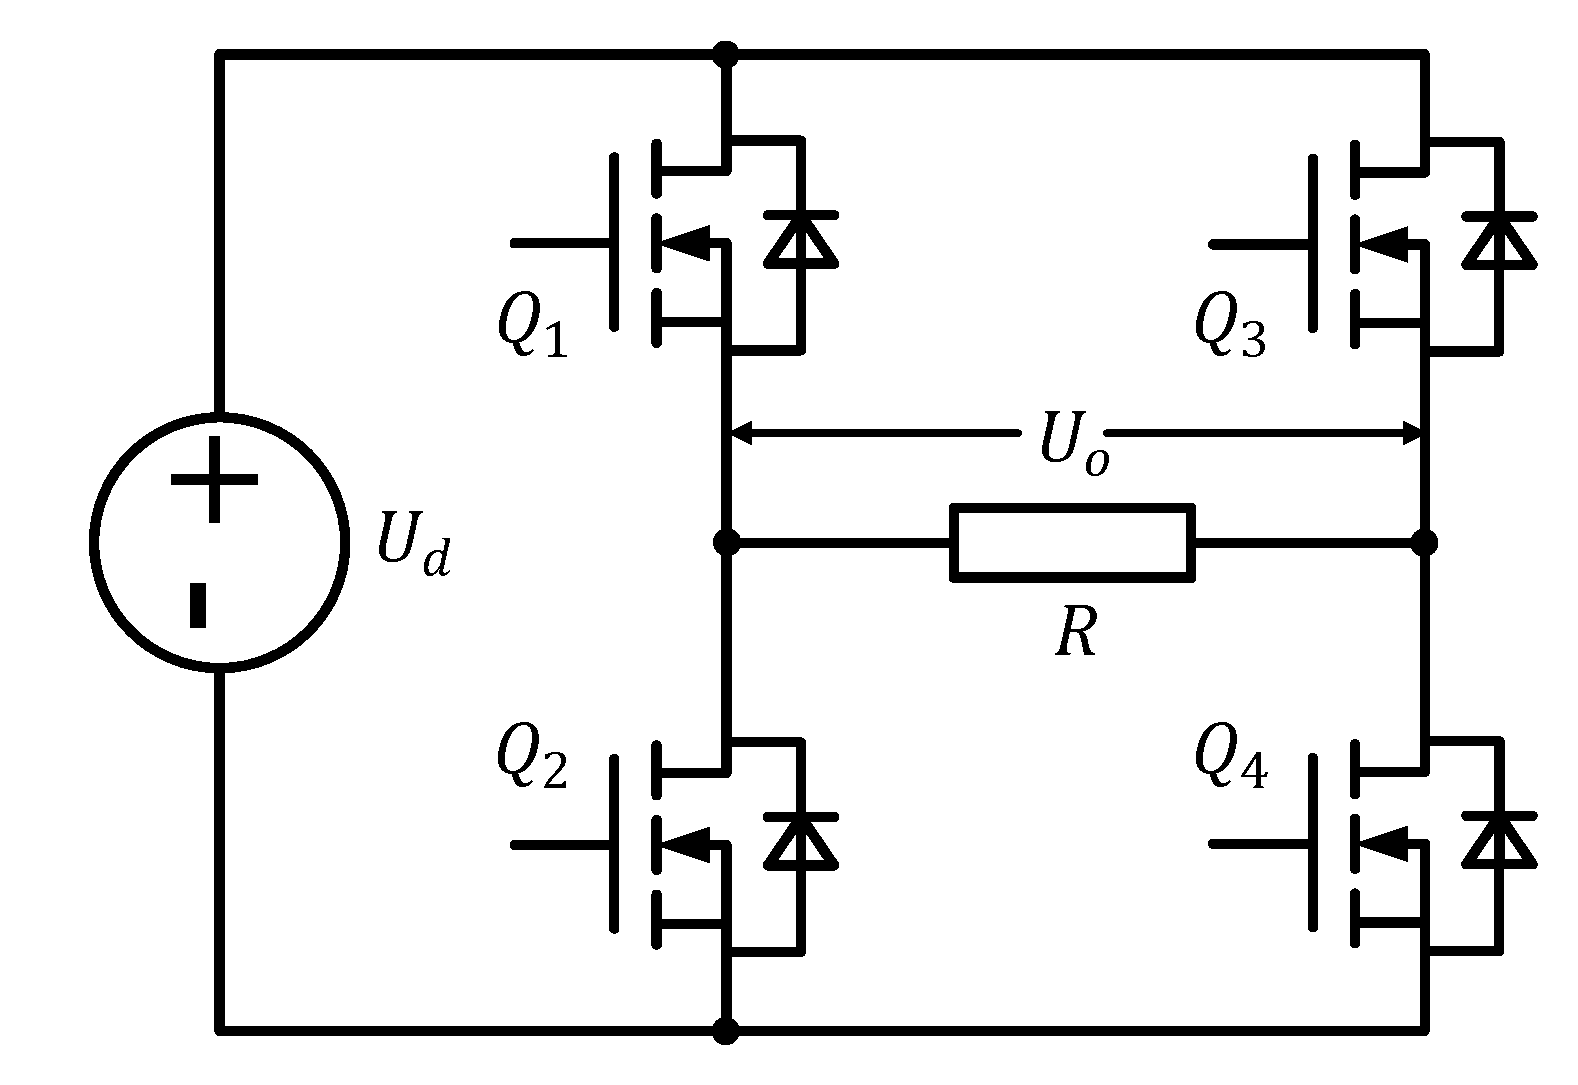
\includegraphics[scale=0.23]{Fig/fullbridge.pdf}
\end{minipage}\\[1pt]
\begin{minipage}[t]{0.5\textwidth} % 以下为新添加页面划分，[t]表示行顶部对齐
\caption{\label{halfbridge}半桥逆变器拓扑结构}
\end{minipage}%
\begin{minipage}[t]{0.5\textwidth}
\caption{\label{fullbridge}全桥逆变器拓扑结构}
\end{minipage}%
\end{figure}

在单相逆变电路中，典型的拓扑结构主要包括桥式型逆变器、变压器能量传递型逆变器以及谐振型逆变器三类。桥式型逆变器是应用最广泛的经典拓扑，其基本原理是通过功率开关器件构成桥臂结构，实现输出电压极性的周期性切换。根据桥臂数量的不同一般可分为半桥逆变器和全桥逆变器，其结构分别如图\ref{halfbridge}和图\ref{fullbridge}所示。半桥逆变器由两个功率开关管互补驱动，输出电压幅值受限于直流母线电压的一半，常应用于中小功率电源中；全桥逆变器由四个功率开关管组成，工作工程中对角器件交替导通，可实现母线电压全幅输出，具有较强的功率输出能力，但因其开关管需同步控制，驱动电路结构相对复杂。

\begin{figure}[htbp]
\centering
\begin{minipage}[c]{0.5\textwidth}
\centering
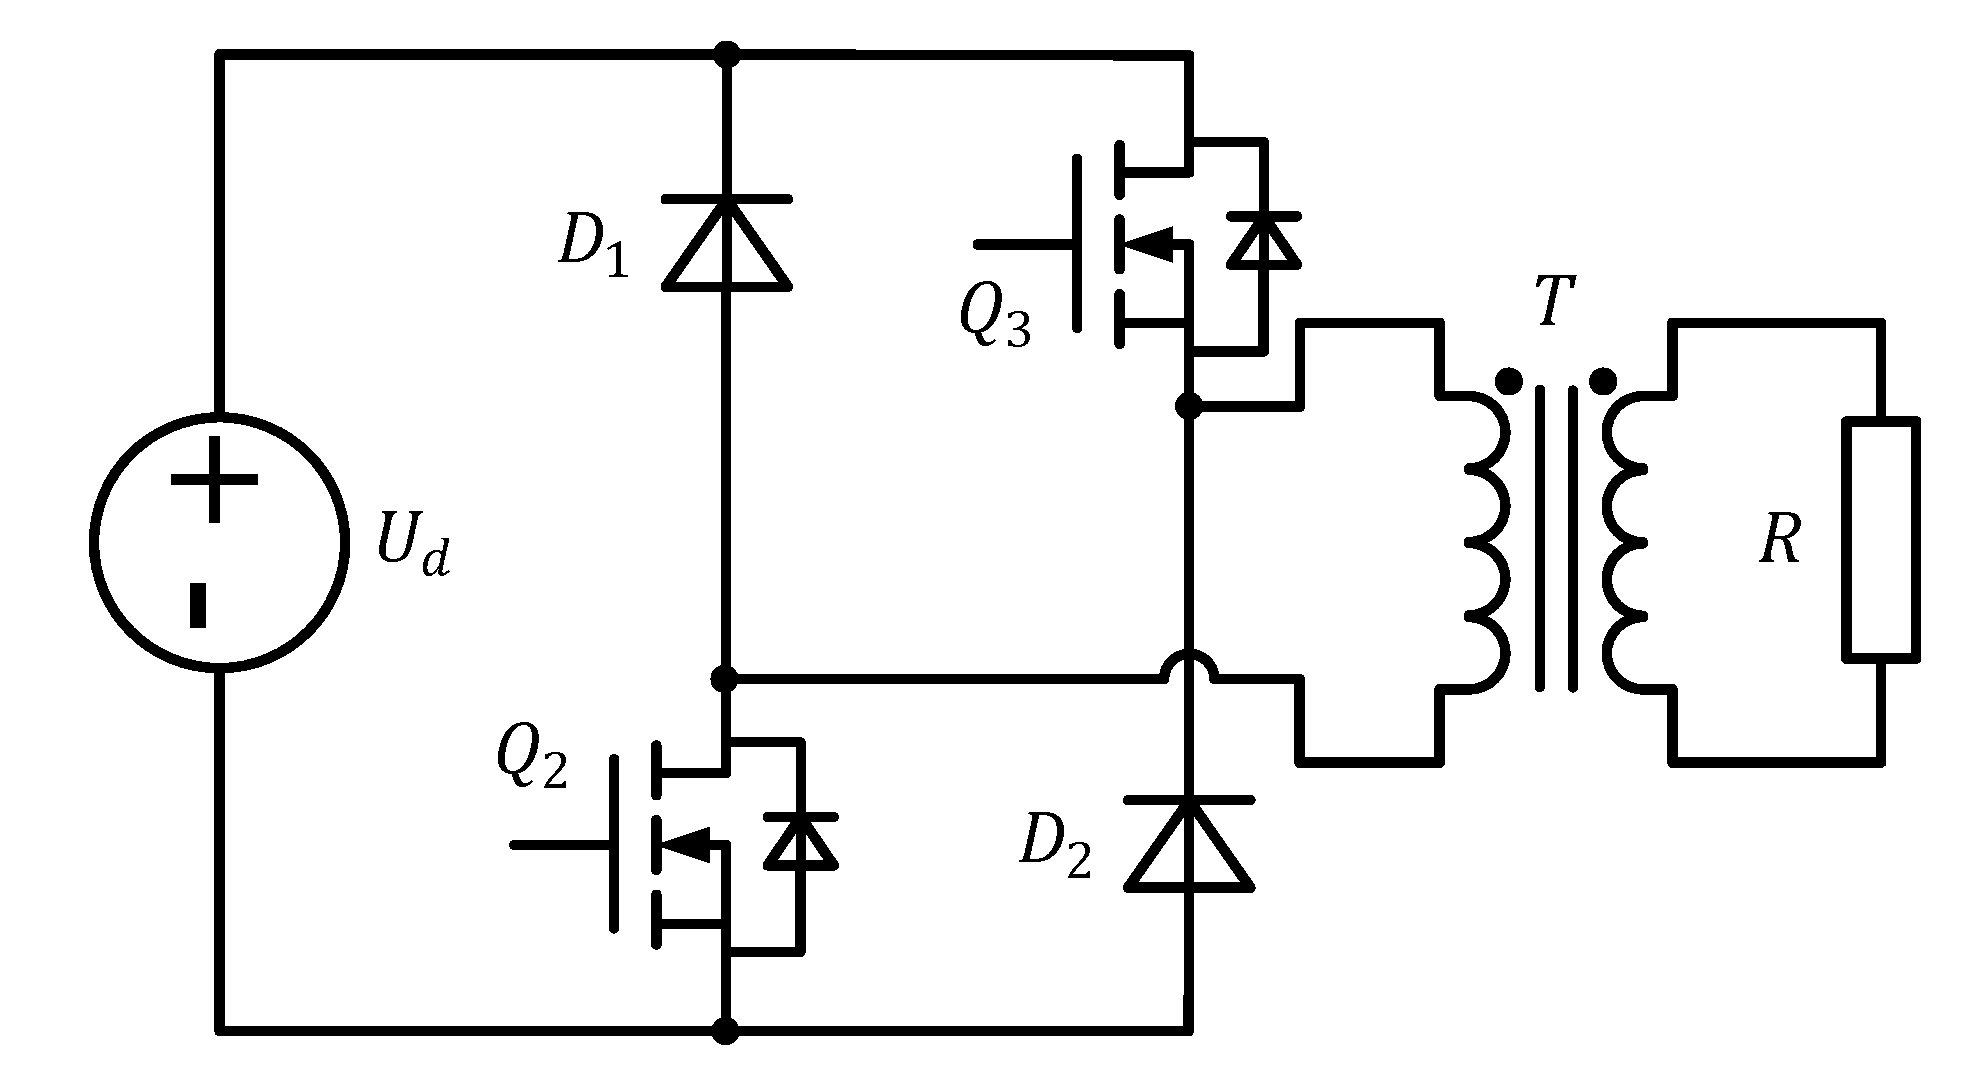
\includegraphics[scale=0.23]{Fig/2tube.pdf} %1:1导入
\end{minipage}%
\begin{minipage}[c]{0.5\textwidth}
\centering
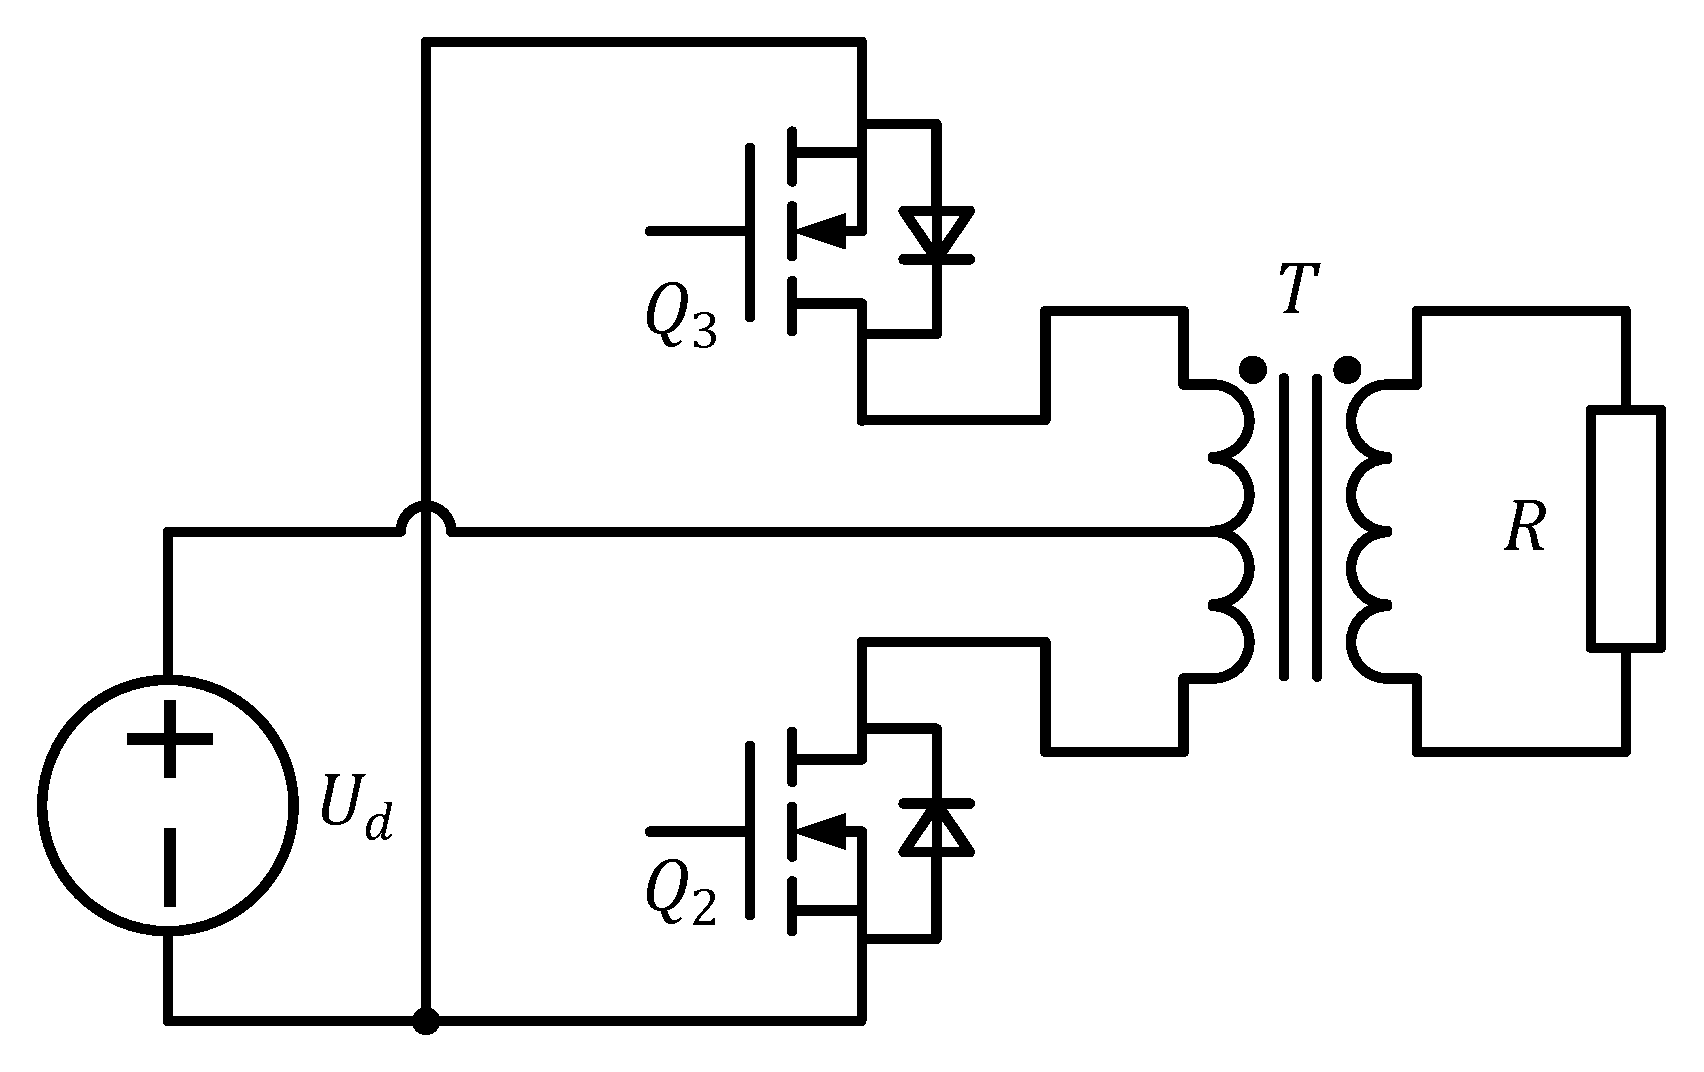
\includegraphics[scale=0.23]{Fig/pushpull.pdf}
\end{minipage}\\[1pt]
\begin{minipage}[t]{0.5\textwidth} % 以下为新添加页面划分，[t]表示行顶部对齐
\caption{\label{2tube}双管正激逆变器拓扑结构}
\end{minipage}%
\begin{minipage}[t]{0.5\textwidth}
\caption{\label{pushpull}推挽逆变器拓扑结构}
\end{minipage}%
\end{figure}

变压器能量传递型逆变器由于引入高频变压器，在结构上天然具备电气隔离能力，该类拓扑的核心特征在于通过开关器件控制磁通的建立和复位，使得能量以磁能形式在原边和副边存储与释放。常见的子拓扑包括双管正激逆变器和推挽逆变器，其结构分别如图\ref{2tube}和图\ref{pushpull}所示。双管正激逆变器采用两个功率开关管与两个二极管连接在变压器原边，当开关管$Q_1$，$Q_2$同时导通时，直流母线电压通经变压器耦合向负载传递；当开关管同时关断时，变压器原边磁化电流经过二极管$D_1$，$D_2$续流，负载侧电压为零，能量仅在开关导通期间传递。由此可见，该拓扑输出为单极性脉冲电压波形，不具备交流对称性，需通过后级谐振滤波网络才能获得高频正弦波输出。同时，由于变压器磁通仅在磁滞回线的单一象限内变化，磁芯的有效磁通摆幅较双极性励磁结构显著减小，在相同磁芯和工作频率条件下可传输功率受限，因此通常用于中小功率场合。

推挽逆变器通过两个功率开关管交替导通，驱动中心抽头变压器原边两侧交替励磁，从而在负载侧感应出双极性脉冲电压，具有良好的交流对称性，且变压器磁芯在正负两个象限内交替工作，能够充分利用磁芯的有效磁通摆幅，从而提升功率传输能力。推挽逆变器结构相对简洁，驱动电路实现难度较低，且使用元器件数量较少，但其存在开关管直通短路的风险，需在驱动信号中合理设置死区时间。此外，推挽逆变器的开关器件在关断时需承受两倍直流母线电压的电压应力，对器件耐压等级及电源设计提出了更高要求。

\begin{figure}[htbp]
\centering
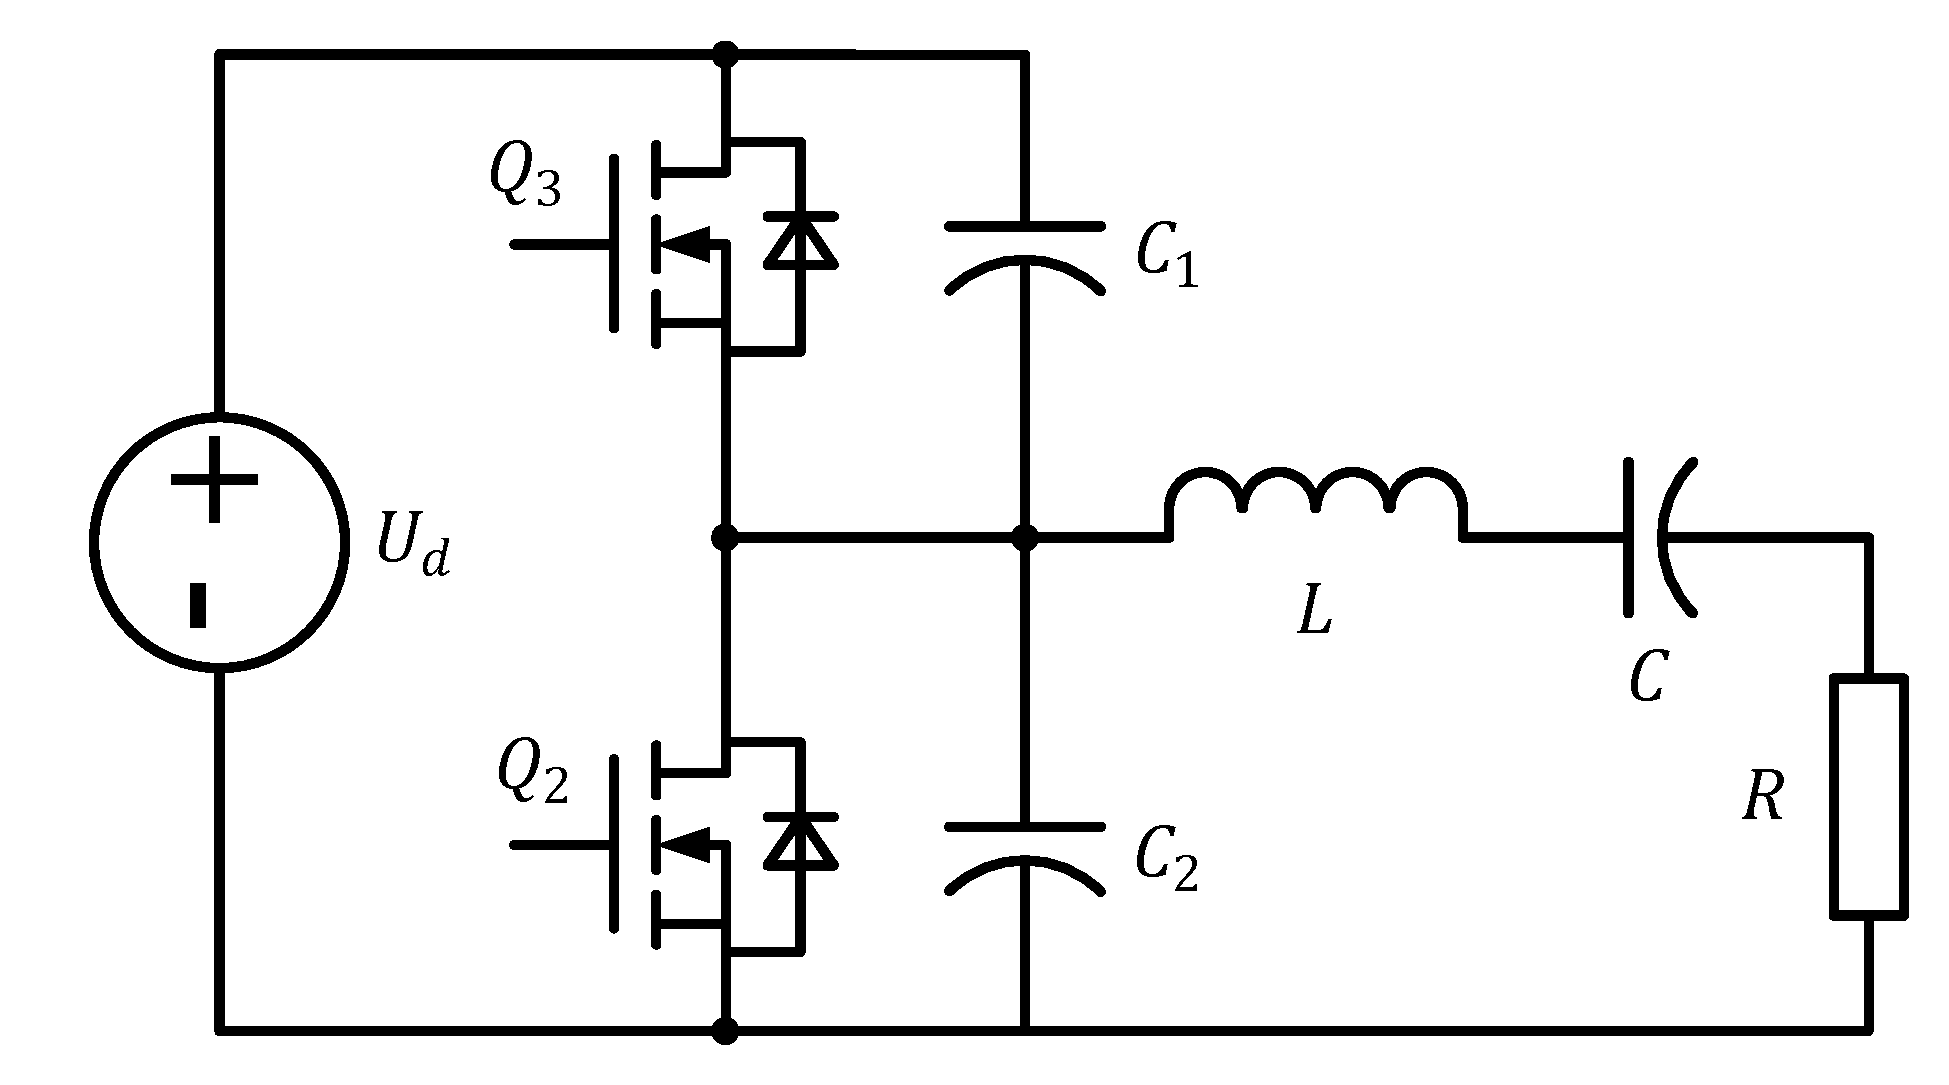
\includegraphics[scale=0.23]{Fig/resonance.pdf}
\caption{\label{resonance}谐振逆变器拓扑结构}
\end{figure}

谐振式逆变器在负载前级引入LC谐振网络，一方面利用谐振特性实现对输出波形的选频与滤波，另一方面使功率开关器件的电压电流波形由谐振特性主导，而非完全由硬开关过程强制切换决定，从而显著降低高频条件下的开关损耗与电磁干扰。典型的DE类逆变器结构如图\ref{resonance}所示，其电路结构与D类逆变器极其类似，不同之处在于两个功率开关管两端增加了并联电容。在占空比为0.25、相位差为180°的工况条件下，两个开关管在同时关断期间输出端并联电容进行充放电过程，使开关管在导通时刻实现零电压开通(ZVS)和零电压导数开通(ZDS)，有效降低高频下的开关损耗，同时也解决了E类逆变器中存在的开关管电压应力较高的问题，在器件选型上可采用耐压等级更低、导通电阻更小的功率器件，有利于减小导通损耗。然而，该类拓扑依赖器件并联电容、外加谐振网络与负载阻抗的参数精确匹配来满足软开关条件，当工作点或负载条件发生偏移时开关应力和损耗会迅速上升，因此更适用于负载特性相对稳定的高频能量场合。

综合比较上述五种逆变电路，考虑高频电外科发生器系统工作频率高、需具备较宽的输出功率调节范围，负载特性变化范围大以及系统实现复杂度等工程需求，本文最终选用推挽逆变器作为系统的高频逆变电路。推挽逆变器结构简单，在功率能力、磁芯利用率、控制复杂度与负载适应性之间取得了较为合理的平衡，能够满足高频电外科发生器电源要求。

\section{系统方案设计}
\begin{figure}[htbp]
% 该图片比例为多次调试过后的最大值，再大就要溢出了
\centering
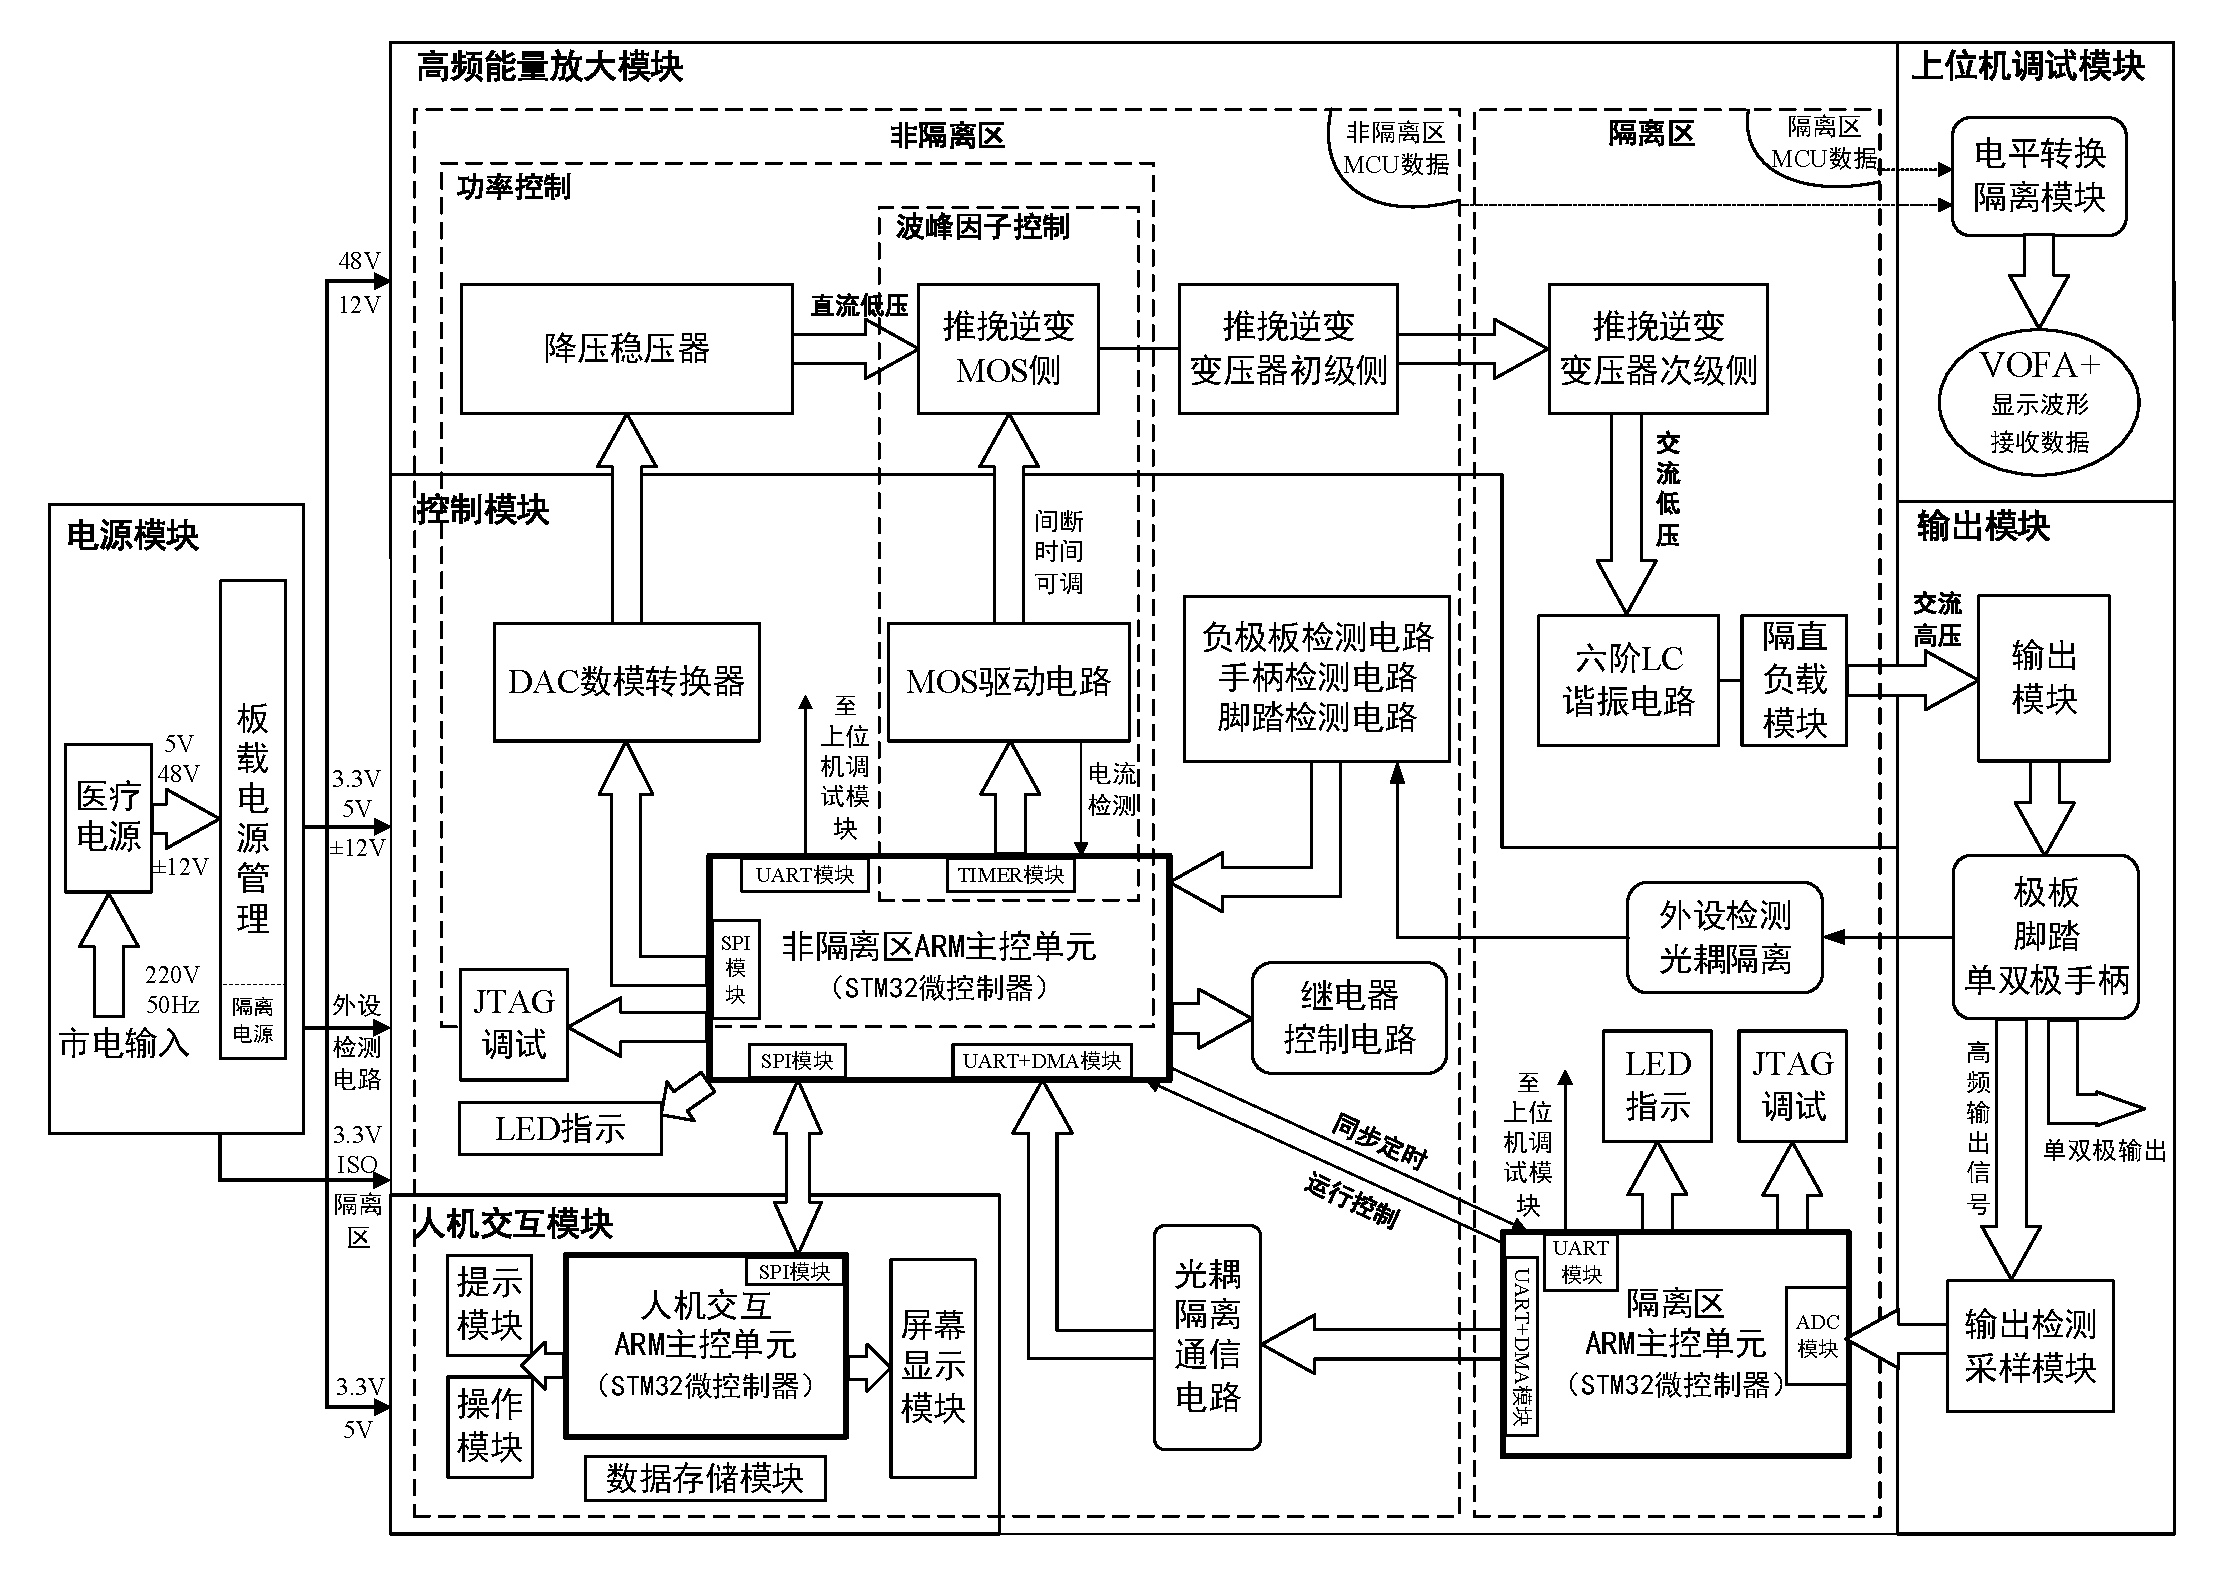
\includegraphics[scale=0.443]{Fig/system.pdf}
\caption{\label{system}系统整体方案设计}
\end{figure}

为实现前文所述设计指标和功能要求，本文设计的高频电外科发生器系统整体设计方案框图如图\ref{system}所示。结合前文对系统调功方式及高频逆变电路拓扑结构的分析，能量发生主电路采用直流调压-推挽逆变的总体结构：交流市电经电源模块中的医疗级开关电源变换后得到48V的直流输出电压，随后通过可调降压稳压电路将其转换为0~48V连续可调的直流电压，并馈入推挽逆变电路，推挽逆变器通过控制开关管的交替导通，实现对直流电能的高频逆变，输出频率为350KHz的脉冲方波电压，同时变高频压器在该过程中提供必要的电气隔离。逆变输出的高频脉冲信号经谐振网络进行选频与滤波后，形成高频正弦电压，并最终输出至手术电极，以完成对生物组织的高频能量传递。

从整体组成上看，该系统主要由电源模块、控制模块、高频能量放大模块、输出模块、人机交互模块以及上位机调试模块六个部分组成。电源模块由医疗电源和板载电源管理电路组成，负责将220V交流市电转换为系统各功能模块所需的多路稳定供电电源；控制模块根据设定的输出功率与输出模式对能量发生电路进行驱动，并实现输出功率的闭环调节，同时对系统外设连接状态及运行状态进行监测；高频能量放大模块作为系统的核心能量转换回路，用于将低压直流电能转换为满足手术需求的高频高压电能；输出模块负责将高频电能隔离输出至手术电极，并完成输出电压、电流的采样和保护功能；人机交互模块用于接收操作者的控制指令，并通过声、光及图像的形式对系统运行状态进行反馈；上位机调试模块通过与系统控制单元建立通信，在系统开发、调试与维护阶段用于辅助参数配置、状态监测及运行调试。

此外，根据系统各功能模块对地电位的不同，可将系统核心模块划分为非隔离区与隔离区两部分。其中，非隔离区内的各模块主要承担系统控制、驱动和人机交互等功能；隔离区内的各模块则直接与输出模块相连，用于对隔离输出的高频信号进行采样与信号传输。非隔离区与隔离区通过隔离变压器及光耦器件实现电源与信号的隔离传输，确保系统的安全可靠运行。

在系统架构层面，由于输出采样模块位于隔离区，而能量发生主电路的驱动与功率控制位于非隔离区，为实现闭环功率控制和输出信号采样选择，采样部分模块需与控制部分模块进行实时交互。因此，本文采用双MCU同步系统架构，将两个MCU分布在不同的隔离区域内，各自承担相应的控制和采样任务，并通过光耦隔离通信模块实现数据与控制信号的可靠传输。同时，通过同步机制对二者任务的执行时序进行协调，以保证系统闭环控制的实时性与稳定性。相关系统实现细节将在后续章节中进一步展开论述。

\section{本章小结}


